\documentclass{ximera}

\input{../preamble}
\author{Ivo Terek}
\license{Creative Commons Attribution-ShareAlike 4.0 International License}
\acknowledgement{}

%Sources: Stitz-Zeager

\title{Vertical and Horizontal Shifts}

\begin{document}
\begin{abstract}
  
\end{abstract}
\maketitle
\licenseSZ

%\typeout{************************************************}
%\typeout{Motivating Questions}
%\typeout{************************************************}

\begin{motivatingQuestions}\begin{itemize}
\item By adding a constant $a$ to a function $f(x)$, what is the relation between the graphs of $y=f(x)$ and $y = f(x)+a$?
\item By performing a ``change of variable'' $x \mapsto x-a$, what is the relation between the graphs of $y=f(x)$ and $y=f(x-a)$?
\item How to use this new understanding to gain a deeper understanding of graphs of quadratic functions (i.e., parabolas)?
\end{itemize}\end{motivatingQuestions}


%\typeout{************************************************}
%\typeout{Subsection Introduction}
%\typeout{************************************************}

\section{Introduction}

Let's consider the two quadratic functions $f(x) = x^2$ and $g(x) = x^2-2x+1$, defined for all real values of $x$. We know what their graphs look like:

  \begin{image}
 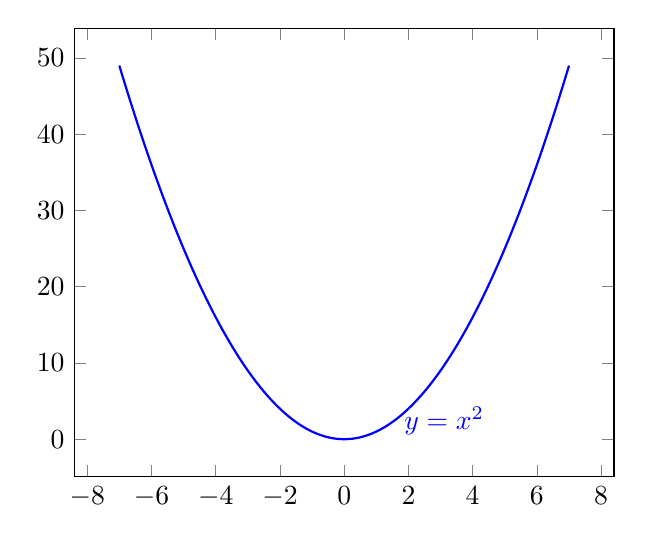
\begin{tikzpicture}
     \begin{axis}
       \addplot[samples=200,thick,domain=-7:7, color=blue]{x^2} node[pos=0.53,right]{\text{$y=x^2$}};
       %\addplot[samples=200,domain=-7:7, color=red]{(x-1)^2};
     \end{axis}
 \end{tikzpicture}
\end{image}
  \begin{image}
 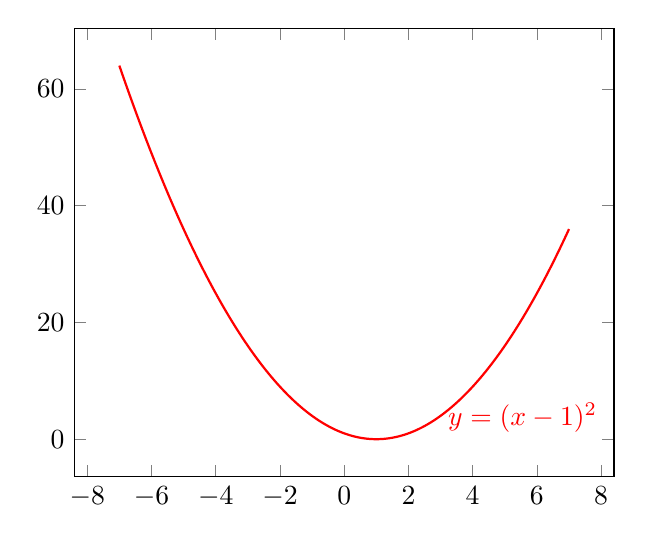
\begin{tikzpicture}
     \begin{axis}
      % \addplot[samples=200,domain=-7:7, color=blue]{x^2};
       \addplot[samples=200,thick, domain=-7:7, color=red]{(x-1)^2} node[pos=0.68,right]{\text{$y=(x-1)^2$}};
     \end{axis}
 \end{tikzpicture}
 \end{image}

The graphs are very similar, down to the horizontal ``width''. In fact, drawing them together, we may see that they only differ by a horizontal translation:

  \begin{image}
 \begin{tikzpicture}
     \begin{axis}
       \addplot[samples=200, thick, domain=-7:7, color=blue]{x^2} node[pos=0.457,left]{\text{$y=x^2$}};
       \addplot[samples=200, thick, domain=-7:7, color=red]{(x-1)^2} node[pos=0.68,right]{\text{$y=(x-1)^2$}};
       \addplot[dashed, thick, color=penColor] coordinates {(1,-7) (1,7)};
     \end{axis}
 \end{tikzpicture}
 \end{image}

Algebraically, one can see that this happens because $$g(x) = x^2-2x+1 = (x-1)^2 = f(x-1).$$
This hints at the following general fact: doing horizontal shifts to the graph of a function amounts to replacing $x$ with ``$x \pm {\rm shift}$'' inside $f(\cdot)$. In this unit, we'll understand in more detail how to work with this, and also how to deal with vertical shifts, as opposed to horizontal shifts. Since vertical shifts are much easier to understand, that's where we'll begin.

\section{Shifting a function vertically}

Let's consider a very simple situation, where we have two functions $f(x) = x^2$ and $g(x) = x^2+4$. Graphing them, in order, we have that

  \begin{image}
 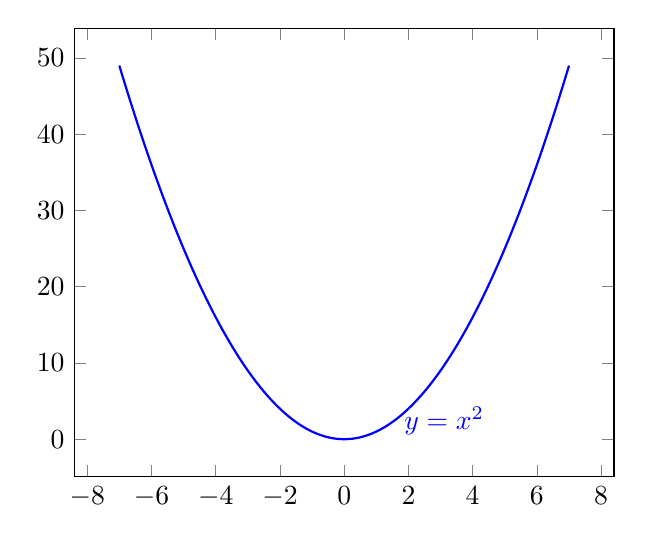
\begin{tikzpicture}
     \begin{axis}
       \addplot[samples=200, thick, domain=-7:7, color=blue]{x^2} node[pos=0.53,right]{\text{$y=x^2$}};
       %\addplot[samples=200,domain=-7:7, color=red]{(x-1)^2};
     \end{axis}
 \end{tikzpicture}
\end{image}
  \begin{image}
 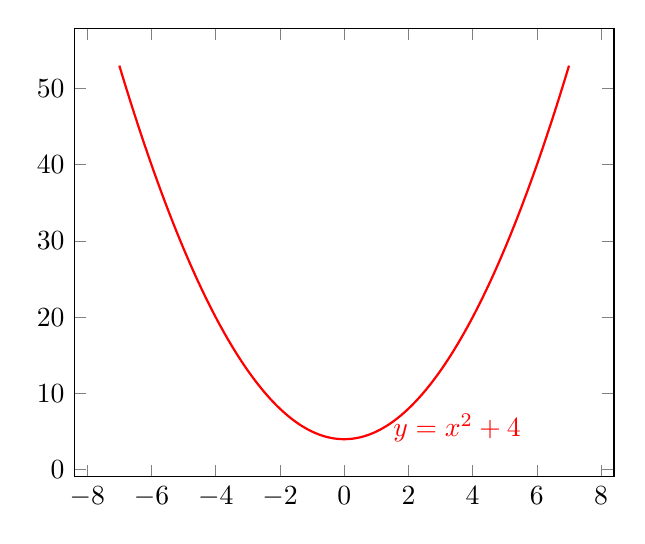
\begin{tikzpicture}
     \begin{axis}
      % \addplot[samples=200,domain=-7:7, color=blue]{x^2};
       \addplot[samples=200, thick,domain=-7:7, color=red]{x^2+4} node[pos=0.52, right]{\text{$y=x^2+4$}};
     \end{axis}
 \end{tikzpicture}
 \end{image}

 Clearly, $f(x)$ and $g(x)$ are directly related via $g(x) = f(x)+4$, and seeing their graph together, we have that:

   \begin{image}
 \begin{tikzpicture}
     \begin{axis}
       \addplot[samples=200,thick,domain=-7:7, color=blue]{x^2} node[pos=0.53,right]{\text{$y=x^2$}};
       \addplot[samples=200,thick,domain=-7:7, color=red]{x^2+4} node[pos=0.52, right]{\text{$y=x^2+4$}};
       \addplot[dashed, thick,, domain=-7:7, color=penColor]{4};
     \end{axis}
 \end{tikzpicture}
 \end{image}

In other words, the graph of $y=g(x)$ was obtained from the graph of $y=f(x)$ by shifting it up exactly by $4$ units. This is a very general phenomenon, that happens for any functions who differ by a constant.

\begin{callout}
  {\bf Theorem (vertical shifts):} Suppose $f$ is a function and $a$ is a positive number.
  \begin{itemize}
  \item To graph $y = f(x)+a$, shift the graph of $y=f(x)$ up $a$ units, by adding $a$ to the $y$-coordinates of the points on the graph of $f$.
      \item To graph $y = f(x)-a$, shift the graph of $y=f(x)$ down $a$ units, by subtracting $a$ from the $y$-coordinates of the points on the graph of $f$.
  \end{itemize}
\end{callout}

In the above setting, it is useful to call $f$ the {\bf parent function}.

\begin{callout}
  {\bf Convention:} Here, we'll always draw graphs of parent functions in blue, and graphs of the ``child'' functions in red. We'll indicate with a dashed line where the shift has happened.
\end{callout}

\begin{example}
  For each of the following functions, find the parent function. How would the graph look like, in terms of the graph of the original function?
  \begin{enumerate}[label=\alph*.]
  \item $g(x) = 2e^{-x} - 1$. \\[.5em]
    \begin{explanation}
      Setting $f(x) = 2e^{-x}$, we have that $g(x) = f(x)-1$. So, to graph $y=g(x)$, we just need to consider the graph of $y=f(x)$ and shift it one unit down.
      \begin{image}
        \begin{tikzpicture}
          \begin{axis}
            \addplot[samples=200,thick,domain=-3:7, color=blue]{2*exp(-x)} node[pos=0.95,above]{\text{$y=2e^{-x}$}};
            \addplot[samples=200,thick,domain=-3:7, color=red]{2*exp(-x)-1} node[pos=0.95,below]{\text{$y=2e^{-x}-1$}};
            \addplot[dashed, thick, domain=-7:7,color=penColor]{1};
          \end{axis}
        \end{tikzpicture}
      \end{image}
    \end{explanation}
  \item $g(x) = \sin(x) + 2$. \\[.5em]
    \begin{explanation}
      Here, we can just recognize that for $f(x) = \sin(x)$, we have $g(x) = f(x)+2$. Thus, we just need to shift the graph of $y=\sin(x)$ up by $2$ units.
      \begin{image}
        \begin{tikzpicture}
          \begin{axis}
            \addplot[samples=200,thick,domain=-7:7, color=blue]{sin(deg(x))} node[pos=0.85,below]{\text{$y=\sin(x)$}};
            \addplot[samples=200,thick,domain=-7:7, color=red]{sin(deg(x))+2} node[pos=0.65,above]{\text{$y=\sin(x)+2$}};
            \addplot[dashed, thick, domain=-7:7,color=penColor]{2};
          \end{axis}
        \end{tikzpicture}
      \end{image}
    \end{explanation}
  \item $g(x) = 2x-3$ \\[.5em]
    \begin{explanation}
      Granted, graphing a linear function poses little to no challenge, but understanding how things work in this setting might offer us some general insight on $y$-intercepts. If $f(x) = 2x$, then $g(x) = f(x)-3$. Graphing $g(x) = 2x$ is easier than easy: just a line with slope $2$ passing through the origin. And the shift down by $3$ units comes last, as you would expect:
            \begin{image}
        \begin{tikzpicture}
          \begin{axis}
            \addplot[domain=-7:7, thick, color=blue]{2*x} node[pos=0.7, left]{\text{$y=2x$}};
            \addplot[domain=-7:7, thick, color=red]{2*x-3} node[pos=0.7, right]{\text{$y=2x-3$}};
            \addplot[dashed, thick, domain=-7:7,color=penColor]{-3};
          \end{axis}
        \end{tikzpicture}
      \end{image}
    \end{explanation}
  \end{enumerate}
\end{example}


\section{Shifting a function horizontally}

Consider again the example given in the introduction, where we have $f(x) = x^2$ and $f(x-1) = x^2-2x+1$. The first thing we would like to address is a source of frequent confusion when first learning this topic. Namely, we have replaced $x$ with $x-1$ in the formula for $f(x)$, but the graph of the modified function ended up shifted to the \emph{right}, even though one might expect the shift to have happened to the \emph{left}, due to the negative sign in the $x-1$ factor!

Here is one safe way to think about it: imagine that you are standing on the $x$-axis and, say, at the origin of the cartesian plane, but that the graph of $y=f(x)$ is already drawn. Replacing $x$ with $x-1$ \emph{does move} the $x$-axis to the left. But \emph{you, the observer}, standing on the $x$-axis, sees the graph move to the right!

Alternatively, compare this with what happened with vertical shifts, but switching the roles of the $x$-axis and $y$-axis. More precisely, start with the graph of $y=f(x)$, then rotate it by $90^\circ$ clockwise (this switches the axes). Replacing $x$ with $x-1$ now brings the graph down by $1$ unit. Finally, rotate everything back by $90^\circ$ counterclockwise (this undoes the switching of the axes). The resulting graph is obtained from the original one by shifting it to the \emph{right}, not left. 

\begin{callout}
  {\bf Theorem (horizontal shifts):} Suppose $f$ is a function and $a$ is a positive number.
  \begin{itemize}
  \item To graph $y = f(x-a)$, shift the graph of $y=f(x)$ right $a$ units, by adding $a$ to the $x$-coordinates of the points on the graph of $f$.
      \item To graph $y = f(x+a)$, shift the graph of $y=f(x)$ left $a$ units, by subtracting $a$ from the $x$-coordinates of the points on the graph of $f$.
  \end{itemize}
\end{callout}

As before we'll continue to call $f$ the {\bf parent function}, whose graph will be drawn in blue, while the graphs of the ``child'' functions will be indicated in red.

\begin{example}
  For each of the following functions, find the parent function. How would the graph look like, in terms of the graph of the original function?
  \begin{enumerate}[label=\alph*.]
  \item $g(x) = 4e^{x+3}$. \\[.5em]
    \begin{explanation}
      Here, if we look at $f(x) = 4e^x$, then we have that $g(x) = 4e^{x+3} = f(x+3)$. So, to graph $y=g(x)$, we may just graph $y = f(x)$, and then shift it $3$ units to the left.
      \begin{image}
        \begin{tikzpicture}
          \begin{axis}
           \addplot[samples=200,thick,domain=-7:3, color=blue]{4*exp(x)} node[pos=0.11, right]{\text{$y=4e^x$}};
           \addplot[samples=200,thick,domain=-7:2, color=red]{4*exp(x+3)} node[pos=0.01, left]{\text{$y=4e^{x+3}$}};
         \addplot[dashed, thick, color=penColor] coordinates {(-3,-7) (-3,7)};
          \end{axis}
        \end{tikzpicture}
      \end{image}
    \end{explanation}
  \item $g(x) = \sin(x - (\pi/2))$. \\[.5em]
    \begin{explanation}
      Consider this time $f(x) = \sin x$. Then we have that $g(x) = f(x-(\pi/2))$, which means that to graph $y=g(x)$, we may take the graph of $y=\sin x$ and shift it to the right by $\pi/2$ units. We obtain:
            \begin{image}
        \begin{tikzpicture}
          \begin{axis}
            \addplot[samples=200,thick,domain=-7:7, color=blue]{sin(deg(x))} node[pos=0.8, below]{\text{$y=\sin(x)$}};
            \addplot[samples=200,thick,domain=-7:7, color=red]{sin(deg(x - pi/2))} node[pos=0.78, above]{\text{$y=\sin(x-(\pi/2))$}};
            \addplot[dashed, thick, color=penColor] coordinates {(pi/2,-7) (pi/2,7)};
          \end{axis}
        \end{tikzpicture}
      \end{image}
      You might be thinking now that the graph of $y = \sin(x-(\pi/2))$ looks an awful lot like the graph of $y = -\cos x$. This is not a coincidence and indeed $\sin(x-(\pi/2)) = -\cos x$ is true for all values of $x$. We will explore such relations (and more) between trigonometric functions, in future units.
    \end{explanation}
  \item $g(x) = (x-2)^2 - 5(x-2)+6$. \\[.5em]
    \begin{explanation}
      As you might be guessing by now, the parent function can be found by just seeking the shifted variable (in this case, $x-2$), and replacing it with $x$. Meaning that if $f(x) = x^2-5x+6$, then $g(x) =f(x-2)$. Thus, to graph $y=g(x)$, we can just graph $y=f(x)$ and shift it $2$ units to the right. Since we can write $f(x) = (x-2)(x-3)$, we know that $f$ is a parabola which crosses the $x$-axis at $x=2$ and $x=3$, and it is concave up (we'll understand how to graph parabolas in a bit more of detail, finding also its vertex, on the next section). Hence:
      \begin{image}
        \begin{tikzpicture}
          \begin{axis}
            \addplot[samples=200,thick,domain=-7:7, color=blue]{x^2-5*x+6} node[pos=0.775, left]{\text{$y=f(x)$}};
            \addplot[samples=200,thick,domain=-7:7, color=red]{(x-2)^2-5*(x-2)+6}node[pos=0.9, right]{\text{$y=g(x)$}};
            \addplot[dashed, thick, color=penColor] coordinates {(4.5,-7) (4.5,7)};
          \end{axis}
        \end{tikzpicture}
      \end{image}
    \end{explanation}
  \end{enumerate}
\end{example}

\section{More on parabolas}

Let's discuss what happens with parabolas and quadratic functions more precisely. Consider a generic $f(x) = ax^2+bx+c$, with $a$, $b$ and $c$ real numbers, and assume that $a \neq 0$. We assume this because if $a$ were zero, we would have a linear function instead of a quadratic one, which is not the focus here. The quadratic formula $$  x = \frac{-b \pm \sqrt{b^2-4ac}}{2a},$$used to find the values of $x$ for which $f(x) = 0$ or, in other words, the possible $x$-intercepts, is usually a source of grief for people studying quadratic functions for the first time. Let's try to remedy this by understanding where such formula comes from. The main strategy here is a little algebraic device called ``completing the squares'', which is also useful for finding the coordinates $(h,k)$ of the vertex of the parabola given by the graph of $f(x)$.

Very briefly, the procedure consists in noting that $(x-h)^2 = x^2-2hx+h^2$ and paying close attention to the $-2hx$ term. Comparing this with the linear term you were given will tell you what $h$ should be. Add and subtract whatever you need to in the quadratic function you were given, to produce $(x-h)^2$ (or, more generally, the multiple $a(x-h)^2$), and whatever constant term is left outside the factored $(\cdots)^2$ will be the desired $k$. We'll see several examples below.

\begin{example}
  For each of the following quadratic functions, rewrite it in the form $f(x) = a(x-h)^2+k$, for suitable numbers $h$ and $k$. Such point $(h,k)$ is automatically the vertex of the parabola in question.
  \begin{enumerate}[label=\alph*.]
  \item $f(x) = x^2-4x+7$. \\[.5em]
    \begin{explanation}
      Comparing $x^2-4x$ with $x^2-2hx$ suggests that $h=2$ does the trick. Since $h^2=4$, we add and subtract $4$ in the expression for the given $f(x)$, to get $$  f(x) = x^2-4x+7 =(x^2-4x+4)-4+7 = (x-2)^2+3.   $$Hence, the vertex of the parabola $y=x^2-4x+7$ is the point $(2,3)$.
    \end{explanation}
  \item $f(x) = 2x^2 + 6x+12$. \\[.5em]
    \begin{explanation}
      This time, look at $2x^2+6x = 2(x^2+3x)$, and compare $x^2+3x$ with $x^2-2hx$. It seems like $h=-3/2$ is what we need. Note that $h^2 = 9/4$. Because of the $2$ we had to factor out, we'll add and subtract $2 \cdot (9/4) = 9/2$ to complete the square. So \begin{align*}f(x) &= 2x^2+6x+12 = 2x^2+6x + \frac{9}{2} - \frac{9}{2} + 12 \\ &= 2\left(x^2+3x+\frac{9}{4}\right) -\frac{9}{2} + 12 = 2\left(x+\frac{3}{2}\right)^2 + \frac{15}{2}\\ &=  2\left(x-\left(-\frac{3}{2}\right)\right)^2 + \frac{15}{2}.\end{align*}Thus $(h,k) = (-3/2, 15/2)$ is the vertex of this parabola.
    \end{explanation}
  \item $f(x) = 3x^2 + 12x + 14$. \\[.5em]
    \begin{explanation}
      As before, we start focusing on $3x^2+12x = 3(x^2+4x)$. Compare $x^2+4x$ with $x^2-2hx$ to see that we need $h = -2$ here. Since $h^2 = 4$, let's add and subtract $3 \cdot 4 = 12$ from the original expression, to obtain
      \begin{align*}
        f(x) &= 3x^2+12x+14 = (3x^2+12x+12)-12+14 \\ &= 3(x^2+4x+4) + 2 = 3(x+2)^2+2 \\ &= 3(x-(-2))^2+2.
      \end{align*}
So, the vertex of this parabola has coordinates $(h,k) = (-2,2)$.
    \end{explanation}
  \end{enumerate}
\end{example}

Very generally, consider $f(x) = ax^2+bx+c$, with $a$, $b$ and $c$ real numbers, with $a \neq 0$. Let's repeat everything we have done in the previous example, with $a$, $b$ and $c$ instead of concrete numbers. Here are the steps we can follow:

\begin{itemize}
\item First, look only at $ax^2 + bx = a(x^2 + bx/a)$.
\item Compare $x^2+bx/a$ with $x^2-2hx$. The $h$ we need here is $h = -b/2a$. Note that $h^2 = b^2/4a^2$.
\item Because of the $a$ we had to factor out in the beginning, let's add and subtract $a \cdot (b^2/4a^2) = b^2/4a$ from the original expression.
\item Compute \begin{align*}  ax^2+bx+c &= \left(ax^2+bx + \frac{b^2}{4a}\right) - \frac{b^2}{4a}+c \\ &= a\left(x^2+\frac{bx}{a} + \frac{b^2}{4a^2}\right) + \frac{-b^2+4ac}{4a} \\ &= a\left(x+\frac{b}{2a}\right)^2+\frac{-b^2+4ac}{4a} \\ &= a\left(x - \left(-\frac{b}{2a}\right)\right)^2 + \frac{-(b^2-4ac)}{4a}. \end{align*}
\item Hence, the vertex of the parabola described by $y=ax^2+bx+c$ is given by $$(h,k) = \left(-\frac{b}{2a}, -\frac{b^2-4ac}{4a}\right).$$
\end{itemize}

And with those computations in place, we are in fact very close to understanding where the quadratic formula came from. Solving $ax^2+bx+c=0$ is, by the above, the same as solving $$a\left(x+\frac{b}{2a}\right)^2 - \frac{b^2-4ac}{4a} = 0.$$Reorganize as $$a\left(x+\frac{b}{2a}\right)^2 = \frac{b^2-4ac}{4a},$$and divide by $a$ to get $$\left(x+\frac{b}{2a}\right)^2 = \frac{b^2-4ac}{4a^2}.$$Assuming that $b^2-4ac \geq 0$, we may take square roots on both sides: $$\left|x+\frac{b}{2a} \right| = \frac{\sqrt{b^2-4ac}}{2|a|}.$$
Eliminating the absolute values, we have $$x+\frac{b}{2a} = \frac{\pm\sqrt{b^2-4ac}}{2a}.$$Now solve for $x$, by putting everything on the right side under a common denominator: $$x = \frac{-b\pm \sqrt{b^2-4ac}}{2a}.$$Mystery solved. For each choice of sign $\pm$, we get one $x$-intercept. Now, we also observe that the average of such solutions does give the $x$-coordinate of the vertex, as you might expect: $$\frac{1}{2}\left(\frac{-b-\sqrt{b^2-4ac}}{2a} + \frac{-b+\sqrt{b^2-4ac}}{2a}\right) = \frac{1}{2} \left(\frac{-2b}{2a}\right) = -\frac{b}{2a}.$$

The $y$-coordinate of the vertex will be, naturally, $k = f(-b/2a)$. This can also be used as a shortcut to write quadratic functions in vertex-form.

\begin{example}
  Write $f(x) = x^2 - 8x+15$ in vertex-form $f(x) = a(x-h)^2+k$ without completing the squares explicitly.\\[.5em]
  \begin{explanation}
    We can factor the quadratic as $f(x) = (x-3)(x-5)$. This means that the $x$-coordinate of the vertex is $h = (3+5)/2 = 4$, and so $$k =f(4) = 4^2-8\cdot 4 + 15 = -1.$$Hence $x^2-8x+15 = (x-4)^2-1$. As a quick sanity-check (particular to \emph{this} example), note that factoring this last result as a difference of squares (because $1^2=1$) does give $(x-3)(x-5)$.
  \end{explanation}
\end{example}

%\typeout{************************************************}
%\typeout{Summary}
%\typeout{************************************************}

\begin{summary}\begin{itemize}
\item Vertical shifts: given the graph of $y=f(x)$, we can draw the graph of $y=f(x)+a$, with $a>0$, by shifting the graph of $y=f(x)$ up by $a$ units. Similarly, the graph of $y=f(x)-a$ is obtained by shifting the original graph down by $a$ units.
\item Horizontal shitfs: given the graph of $y=f(x)$, we can draw the graph of $y=f(x-a)$, with $a>0$, by shifting the graph of $y=f(x)$ by $a$ units to the left. Similarly, the graph of $y=f(x+a)$ is obtained by shifting the original graph by $a$ units to the right.
\item For an arbitrary quadratic function $f(x) = ax^2+bx+c$, we found formulas for the coordinates $(h,k)$ of its vertex by completing the squares. We have also concluded that the $x$-coordinate $h$ of the vertex is, in fact, the average of the $x$-intercepts of the parabola described as the graph of $y=f(x)$ and, in particular, we have seen how to deduce the famous quadratic formula with this general strategy.
\end{itemize}\end{summary}




\end{document}
